\documentclass[spanish,letterpaper]{templates/uchile-tesis}

% Comandos especiales de esta tesis
%\newcommand{\mb}{\textit{microblogging}\xspace}
%\newcommand{\web}{Web\xspace}
%\newcommand{\tw}{\textit{Twitter}\xspace}
%\newcommand{\etal}{\textit{et. al.}\xspace}

% Portada - Variables
\facultad{Facultad de Ciencias Físicas y Matemáticas} 
\departamento{Departamento de Ingeniería Civil Eléctrica}
\title{Diseño e Implementación de una plataforma para experimentos en microgravedad y de electrónica en ambiente hostil con Nano-Satélites}

\carrera{INGENIERO CIVIL ELÉCTRICO}

\trabajoygrado{MEMORIA PARA OPTAR AL TÍTULO DE
}
%\trabajoysubgrado{Memoria para optar al título de Ingeniero Civil Industrial}


\author{JOSÉ ALBERTO OGALDE ORTIZ}

\profguia{MARCOS DÍAZ QUEZADA} %profesor guia
\profcoguia{CLAUDIO FALC\'ON BEAS} %profesor co-guia
\profint{TOMÁS OPAZO TORO} %profesor integrante
%\profinta{Sr. ZZ ZZ ZZ} %profesor integrante 2, generalemente no es necesario
%\profintb{Sr. ZZZ ZZZ ZZZ} %profesor integrante 3, generalmente no es necesario
%\proyecto{Financiado por el proyecto \#ZZZZ}

\ciudad{Santiago} \pais{Chile} \monthpub{Septiembre} \yearpub{2016}

\begin{document}

% Lista de TODOS y FIXMES, no aparece si es que no hay nada que hacer
\listoftodos
\newpage

%% Portada
\maketitle

% Prefacio
\begin{preface}
% Resumen
%\section{Resumen Ejecutivo}
\begin{myAbstract}
%El estándar CubeSat fue desarrollado para facilitar el desarrollo de pequeños proyectos espaciales con fines investigativos y/o académicos. Esto es una ayuda para la evolución tecnológiuca espacial, ya que es posible testear nuevas tecnologías a bordo de un CubeSat sin los mayores costos que involucran la industria espacial tradicional.
%
%Es bajo esta perspectiva que nace el proyecto SUCHAI dentro de la UNiversidad de Chile. Este proyecto comienza con el lanzamiento de su primer Cubesat de 1U en el año 2016  y con el desarrollo de SUCHAI2 un nano-satélite de 3U. La misión de SUCHAI como SUCHAI2 están orientada al trabajo colaborativo de la industria y academia en orden de acercar el espacio al país.

%El estándar de nanosatélites Cubesat fue pensado para facilitar el desarrollo de pequeños
%proyectos espaciales con fines científicos y educacionales, a un bajo costo y en cortos periodos
%de tiempo. Siguiendo esta línea, la Facultad de Ciencias Físicas y Matemáticas de la Uni-
%versidad de Chile ha impulsado el proyecto SUCHAI, que consiste en implementar, poner en
%órbita y operar el primer satélite desarrollado por una universidad del país. 

Típicamente un satélite es diseñado de manera completa entorno a sus payloads a bordo. Este diseño \textit{payload-céntrico} tiene algunas desventajas, como lo son grandes \textit{budget} y un ciclo de desarrollo más largo. Una forma de resolver este problema es establecer una interfaz estandarizada entre el satélite y los payloads. 

Una interface como tal permite separar las etapas de diseño y operación entre el bus del satélite con el de los payloads. Esto puede facilitar la integración de un mismo payload en múltiples satélites, así como reducir el ciclo de desarrollo total de la misión.

Para evitar estos problemas se plantea una plataforma estandarizada entre payloads y el bus de un satélite, la cual está diseñada para operar en los nano-satélites tipo CubeSat que son los más utilizados en la comunidad académica.

%Typically,  a  complete  satellite  will  be  designed  around  each  payload.  This  has  several 
%drawbacks, such 
%as larger budgets and a longer development cycle. However, it does not need to 
%be  this  way.  A  standardized  payload  interface  can  help  alleviate  these  issues  and  allow  for  a 
%lighter budget and a tighter development schedule.
%To  avoid  these  problems  a  modu
%lar  payload  interface  was  designed  to  support  multiple 
%CubeSat  payloads. A  large  part  of  this  work  involved  designing  the Application  Programming 
%Interface for the payload to interact with the satellites main microprocessor. The motivation for a 
%modular i
%nterface is to reduce the budget and development schedule.

%El paradigma tradicional para el desarrollo de satélites es payload-céntrico, el cual es mucho más optimizado para proyectos tradicionales y grandes. Sin embargo, este paradigma obliga a rediseñar el satélite desde cero cada vez. Para evadir este problema se propone el desarrollo de una arquitectura de payload “SUCHPAY” capaz de soportar múltiples buses tipo CubeSat. 

%SUCHPAY es una arquitectura que contiene tanto componentes de software(PAYSW) como de hardware (SUCHPAYHW). Esta configuración pretende facilitar el desarrollo arbitrario de payloads sobre CubeSats. De esta forma, el diseño de payload está completamente desacoplado del bus y de forma análoga, el bus puede ser diseño sin tener conocimiento de la operación o funcionamiento del payload.

SUCHPAY es una plataforma que implementa tal interfaz entre el bus y un payload abordo. La plataforma provee herramientas de software para el desarrollador de payload con el fin de facilitar la integración del payload hacia el bus del satélite. También se provee una API de comandos para el bus, con la cual se estandariza el tipo de  comunicación entre un payload y el bus del satélite.

A modo de validación de la plataforma, se integran dos payload experimentales que consiten en el estudio de la potencia inyectada en un circuito RC y el estudio del coeficiente de disipasión de energía en microgravedad y ambientes hostiles. Ambos payload se integran en el bus de SUCHAI, un CubeSat de 1U desarrollado por la Universidad de Chile.

\end{myAbstract}
% Pagina Optativa - Dedicatoria
\dedicatoria{Gracias al pulento por su incondicional sabiduría en todo momento}

% Pagina Optativa - Agradecimientos
\section{Agradecimientos}
Muchas gracias al spaghetti volador por su infinita sabiduría.
\begin{flushright}
\makeatletter
	\@author
\makeatother
\end{flushright}

% Indice - General
\tableofcontents

% Indice - Tablas
\listoftables

% Indice - Figuras
\listoffigures

\end{preface}

% Introducción
\chapter{Introducción}
\label{ch:introduction}

%\fillup{1}
%\todo{todo 1} asdfasfsdfsadafs %\missingref{me faltaría una ref!}.
%\todo[inline]{todo 2}

La etapa de diseño consiste en explicitar los requerimientos del sistema y generar una
arquitectura de software que representa de manera conceptual la solución a implementar, en
esta etapa se hace un uso extensivo del concepto de patrones de diseño para conseguir la
solución al problema planteado. Durante la implementación se toma la solución conceptual y
se programa el software utilizando las herramientas adecuadas a la plataforma consiguiendo
una plataforma base que consta de controladores de hardware, sistema operativo y la apli-
1cación específica a la misión. Las pruebas se desarrollan sobre el sistema integrado en sus
tres subsistemas básicos mediante la puesta en funcionamiento del satélite por un tiempo
prolongado usando la técnica denominada hardware on the loop simulation adecuada para
probar sistemas embebidos complejos.



\section{Objetivos Generales}

El principal objetivo de este trabajo es diseñar e implementar una plataforma abierta que sirva como interfaz entre un satelites y sus payloads.  En este contexto, abierta significa que los usuarios tendrán acceso completo a las especificaciones de diseño y que pueden construir, modificar y extender los diseños a su propio gusto.  El hecho de definir una interfaz estándar entre el bus y los payloads, permite acelerar los tiempos de desarrollo para múltiples satélites así como también focalizar el desarrollo de payloads.

\section{Objetivos Específicos}

\section{Estructura} 

%Capitulo 2
\chapter{Marco Teórico}

\todo{todo marco teorico 1}Ver cuales son los documentos que hay eliminar/agregar

\todo{todo marco teorico 2} Ver cuales son los documentos que hay que editar.

\subsection{Sistemas embebidos}
Los computadores personales son utilizados por gran parte de la población dado que se caracterizan por tener capacidad para atender una cantidad importante de procesos dispuestos por un sistema operativo en orden para atender diferentes aplicaciones  del usuario final. Un microcontrolador tambi\'en es un tipo de computador salvo que sus recursos normalmente son más limitados que los de un computador personal. Además, un microcontrolador normalmente tiene más flexibilidad para el uso directo de perif\'ericos y poder comunicarse a nivel de máquina con otro dispositivo electrónico.

Un sistema embebido está compuesto por uno más microcontroladores en conjunto con dispositivos electrónicos con los cuales comunicarse para realizar alguna tarea. 
El hardware que compone a un microcontrolador está fijo, por lo que el desarrollador de sistemas embebidos solamente tiene acceso a la programación de \'este en conjunto con la correcta interconexión con otros dispositivos electrónicos. Debe considerarse que a diferencia de un computador personal, el programa que provee la funcionalidad del microcontrolador se denomina \textit{firmware}, ya que en general es específico para la plataforma de hardware utilizada.

\subsubsection{Microcontroladores PIC}
Este trabajo se concentra en el uso de los microcontroladores PIC desarrollados por la compañía Microchip. La familia de microcontroladores  PIC es bastante amplia adaptándose a un amplio rango de necesidades, la tabla \ref{pic_list} resume las principales características de los diferentes modelos y puede ser utilizada como una guía para determinar el dispositivo adecuado según la aplicación:

% ················ TALBA ·················
\begin{table}[ht!]
	\caption{Resumen de familias de Microchip}\label{pic_list}
	\centering 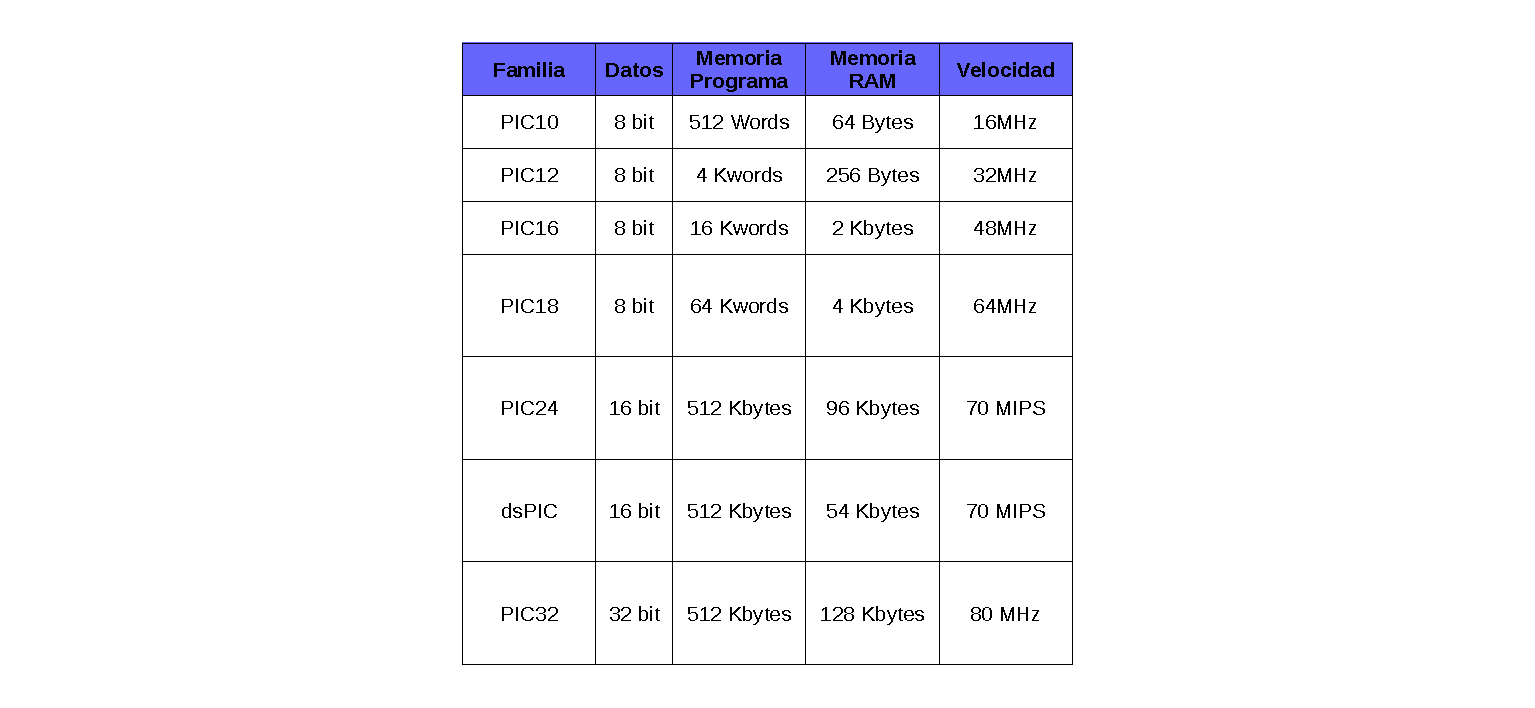
\includegraphics[width=\textwidth]{images/pic_list.pdf}
\end{table}
%··········································
\subsection{Microcontrolador}
Un microcontrolador es un computador pequeño dentro de un solo circuito integrado, que posee un solo nucelo de proceso, memoria y perif\'ericos de entrada/salida. Los microcontroladores estan diseñados para los sistemas embebidos, en contraste a los microprocesadores utilizados en computadores personales u otras aplicaciones de propósito general.

Los microcontroladores son utilizados en dispositivos y productos automáticamente controlados como por ejemplo, controles remotos, sistema de control de automóviles, etc.

\subsection{Nano-Sat\'elites}
Corresponden a los sat\'elites artificiales con una masa entre 1 y 10 kg. Con los continuos avances en la minaturización y capacidad de la electrónica en conjunto al uso de constelaciones de sat\'elites, los nano-sat\'elites están crecientemente capaces de desempeñarse bien en misiones comerciales. Un caso destacable son los nano-sat\'elites que siguen el protocolo CubeSat, cuyo primer lanzamiento fue el 2003 y en el año 2012 se lanzaron 75 sat\'elites al espacio.

\subsubsection{CubeSat}
Es un tipo de nano-sat\'elite hecho de multiples unidades cúbicas de 10x10x10 cm, no tiene más de 1.3 kg de masa por unidad y a menudo utiliza componentes \textit{commercial off-the-shelf} (COTS) para su diseño electrónico y estructura.

Los usos típicos involucran experimentos que pueden ser miniaturizados o experimentos para servir a propósitos como la observación del planeta o comunicación de radio amateur.

Uno de los atractivos de los CubeSats es su bajo costo en comparación a otras tecnologías satelitales. Esto lo convierte en buen candidato para probar nuevas tecnologías a bordo de estas plataformas dado que su costo puede justificar misiones riesgosas.

\subsubsection{Proyecto SUCHAI}
\textit{Satellite of the University of CHile for Aerospace Investigation} (SUCHAI) corresponde al primer sat\'elite artificial diseñado y desarrollado localmente en Chile por un conjunto de estudiantes de pregrado y profesores del Departamento de Ingeniería Elctrica de la Universidad de Chile.
SUCHAI es un nano-sat\'elite de tipo CubeSat de una unidad (aproximadamente 1 kg), cuyo objetivo principal es educacional y científico.
La misión de SUCHAI se considera en los siguientes \textit{payloads}
\begin{itemize}
	\item \textbf{Langmuir probe: } Estudio de la ionósfera en sincronización con el \textit{incoherent scatter radar} (ISR) tomando medidas simultáneas de la variación en la densidad de electrones en la ionósfera.
	\item \textbf{Eletrónica fuera del equilibrio: } Un circuito RC para estudiar las fluctuaciones fuera de equilibrio en la potencia inyectada al estar en un ambiente hostil como el espacio.
	\item \textbf{Experimento termal: } Estudia la disipación de calor en dispositivos electrónicos en un ambiente vacío.
	\item \textbf{Cámara: } Una cámara digital para analizar la factibilidad de observar la tierra desde un cubesat.
	\item \textbf{Receptor GPS: } Un módulo receptor GPS para obtener la posición del sat\'elite y aprender cómo utilizarlo en futuras misiones.
\end{itemize}

\subsubsection{Payload}
Un \textit{payload} es la combinación de hardware y software de una nave espacial que interactúa con un \textit{sujeto} (porción del mundo exterior fuera de la nave espacial), de forma de completar los objetivos de la Misión. Los payloads tipicamente son únicos y específicos para cada misión, dado que son la razón fundamental por la que la nave espacial es lanzada. El propósito del resto de la nave espacial es mantener al payload sano, feliz y apuntando en la dirección correcta.
\subsection{Bus}
Es un dispositivo que actúa como sistema de comunicación entre los componentes de un sistema. En este caso, un bus interconecta todos los módulos de nano-sat\'elite integrando las partes individuales en un sistema completo.
\subsubsection{PC-104}
Es una familia de estándares de sistemas embebidos que define los factores y forma de un bus. El PC-104 está pensado para ambientes especializados donde se necesita un computador pequeño y robusto. El estádar permite diseño modulares y además, posibilita poner placas una de encima de otra en forma de pila.
\subsection{Sensores transductores}
Es un dispositivo que convierte un tipo de energía hacia otra. Usualmente un transducto convierte una señal de un tipo hacia una señal el\'etrica. 
Los transductores son fundamentales en los sistemas de automatización, de medidas y de control, dónde se generan señales el\'etrcias a partir de otras variables físicas (e.g. energía, fuerza, torque, movimiento, posición, etc). Según su uso de potencia, existen transductores activos y pasivos.

\subsection{Actuador}
Es un dispositivo que es responsable de accionar algún tipo de mecanismo sobre un sistema. El tipo de energía utilizado por el actuador es variable (e.g. el\'ectrico, mecánico, químico, etc).
\subsubsection{Conversor ADC}
Un conversor Análogo-a-Digital es un dispositivo que convierte una señal analógica hacia un número digital representado por una señal digital.
\subsubsection{Conversor DAC}
Un conversor Digital-a-Análogo es un dispositivo que convierte un número digital hacia una señal analógica.
\subsection{Controlador de hardware}
Corresponde a un programa/software que manipula o controla un dispositivo de hardware específico. Un driver provee una interfaz de software de manera que el sistema operativo u otro programa pueda acceder a las capacidades del dispositivo de hardware sin necesidad de conocer detalles muy precisos sobre \'este.
\subsection{Microgravedad}
Corresponde a la situación física donde la \textit{ fuerza-g} dada por la ley de gravitación son muy pequeñas, practicamente nulas. Tambi\'en se le conoce como \textit{zero-G} o $\mu g$.
Esta condición se produce por ubicarse a gran distancia de la Tierra o bien encontrarse orbitando la Tierra en caída libre.
\subsection{Sistema fuera de equilibrio}
La termodinámica fuera del equilibrio es una rama de la física que tratacon sistemas y procesos que en general no están en estado de equilibrio termodinámico, pero pueden ser adecuadamente descrito en t\'erminos de variables que son relacionadas con variables de estados termodinámicas.
Un sistema fuera de equilibrio es un sistema que cumple con estos requisitos. Sin embargo, es de particular inter\'es para este trabajo de título, los sistemas que se encuentran en estado estacionario fuera del equilibrio o NESS (NonEquilibrium Steady State).

\subsection{Circuito pasivo}
Corresponde a un circuito el\'ectrico compuesto por elementos discretos que en conjunto consumen energía en vez generarla.
\subsubsection{Circuito RC}
Corresponde a un circuito compuesto por un resistor (R) junto a un capacitor (C). En el desarrollo de este trabajo se refiere a un circuito RC con el resistor y capacitor conectados en serie de forma que forman un filtro pasa bajos.
\begin{figure}[ht!]
	\centering
	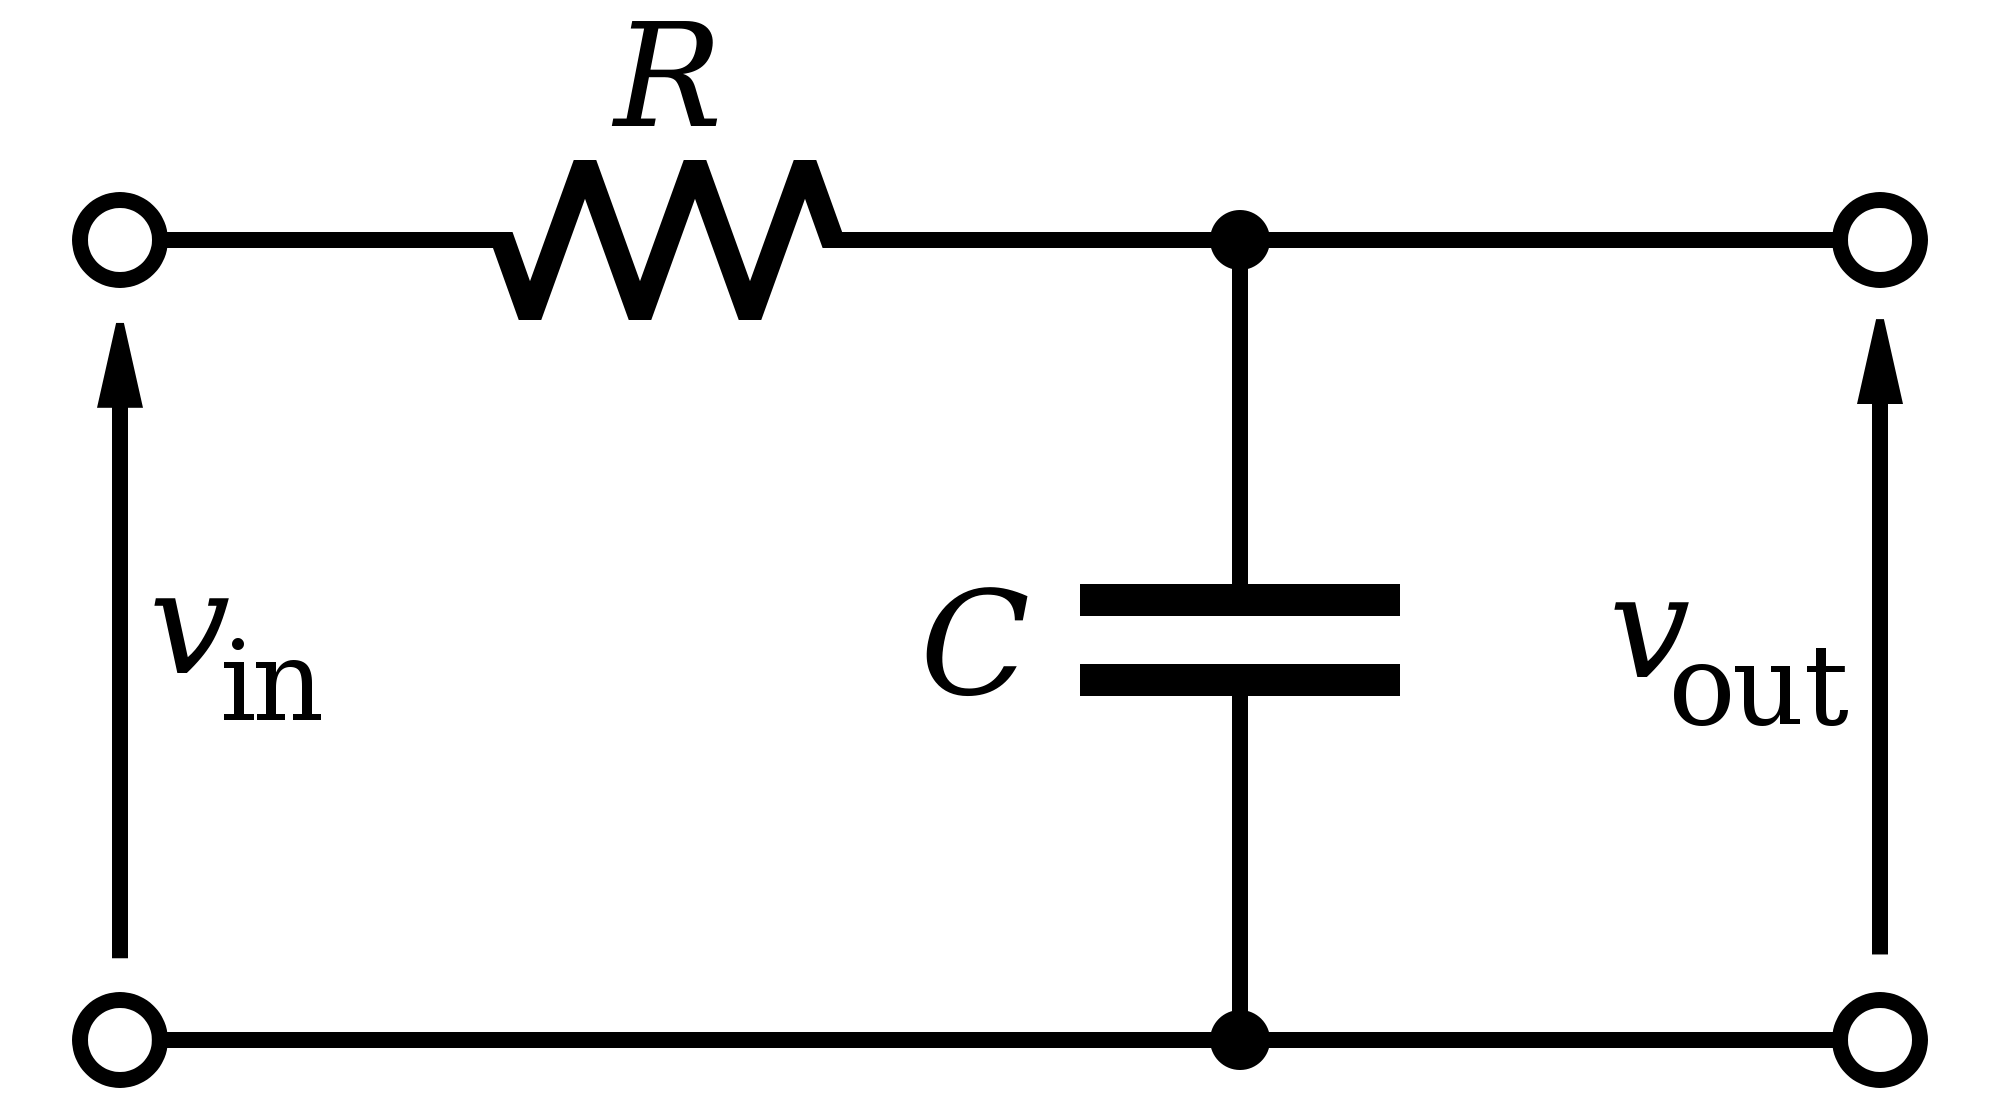
\includegraphics[width=180pt]{images/rc.png}
	\caption{Circuito RC pasa-bajos}
	\label{fig:rc}
\end{figure}

\subsubsection{Filtro pasa bajos}
Corresponde a un dispositivo cuya caracterísitica es bloquear el paso de señales de \textit{alta} frecuencia a la salida del dispositivo, por lo que solamente permite el paso de señales de \textit{baja} frecuencia. Si la señal es una combinación de múltiples señales de diferentes componentes de frecuencias, solamente las componentes de baja frecuencia logran pasar a trav\'es del dispositivo. 

\subsubsection{Potencia inyectada}
Corresponde a la potencia instantánea consumida por un circuito el\'ectrico. 

%Diseño de la interfa
\chapter{Diseño de la plataforma}


\section{Requerimientos}
\subsection{Requirimientos Operacionales}
Se refieren a las funcionalidades que se espera que la plataforma a bordo del satélite debe realizar. Son los requisitos básicos que el sistema debe cumplir para considerar
que se cuenta con una plataforma capaz de llevar a cabo la ejecución y representación del payload. La lista de requerimientos
proviene de una serie de reuniones sostenidas con los integrantes de los diferentes grupos de
trabajo, todo de acuerdo con los lineamientos del jefe de proyecto.

\subsection{Requirimientos No-Operacionales}
Por requerimientos no-operacionales, se entienden aquellos atributos asociados a la calidad de la plataforma, o bien criterios que permiten determinar cómo debería ser la interfaz que se está diseñando. A diferencia de los requerimientos operacionales que explican lo que la plataforma debería hacer, los no funcionales explican las cualidades y restricciones que guiarán el proceso de diseño.

\subsection{Requirimientos mínimos}

\section{Hardware}
\section{Software}
\subsection{Arquitectura del Software}
\subsubsection{API de comunicación}
\subsubsection{SDK para Payloads}
 

%implementacion especifica del diseño
\chapter{Implementación}

% Apéndices
% Adicionales
\begin{additional} 
\section{Capítulo Adicional que no es apéndice}
\end{additional}

% Apéndices
\begin{appendix} 
\section{Tweets}
\end{appendix}



% Bibliografía
\bibliographystyle{abbrv}
\bibliography{../bibliography/tesis}

\end{document}